\section{Bilateral Filter}

\begin{center}
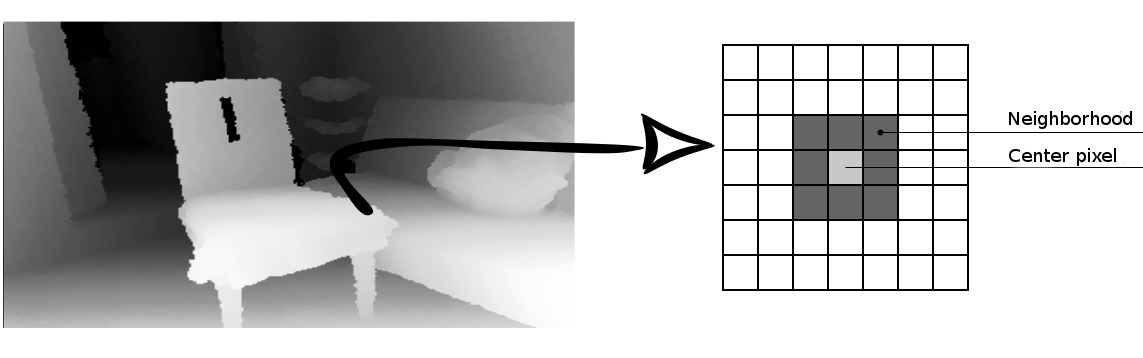
\includegraphics[scale=0.25]{images/vecindarioDepth}
\end{center}

The depthmaps captured by a low cost RGB-D camera usually contains noise, this can be 
consecuence of materials reflectance, device imperfections, object fast movement, distance to the 
sensor, etc. 

In order to reduce the effect of noise is natural to use some kind of filter, as usual in computer 
vision, a typical filter will take information of a pixel and its neighboorhod to generate a result. 
If the image is smooth, without abrupt changes in intensity, a simple average could be enough. However this 
is not the case in the presence of edges or corners, areas where the intensity changes charply. 
The bilateral filter afronts this problem, giving to each neighboor a weight based on its cercany  
to the center pixel. In a grayscale image it takes into account 
the neighboor intensity and distance (in image plane) to calculate the weight. A depthmap is very similar to a grayscale 
image, the only difference is that the depthmap represents geometrical information and usually contains holes 
(areas where the sensor failed to capture distance). 


A bileateral filter was applied to the captures, using the euclidean distance and intensity distance to calculate 
the weight of each pixel neighboor in the depthmap.

In a filter window centered at pixel x, the ponderated average was calculated using the following weight for each neighboor:

$$ kernel(x,sigma) = \frac{e^{-x^2}}{2*\sigma^2} $$

$$ weight = kernel(dist,sigmad)*kernel(intensdist,sigmai) $$

\begin{figure}[h!]
\begin{center}
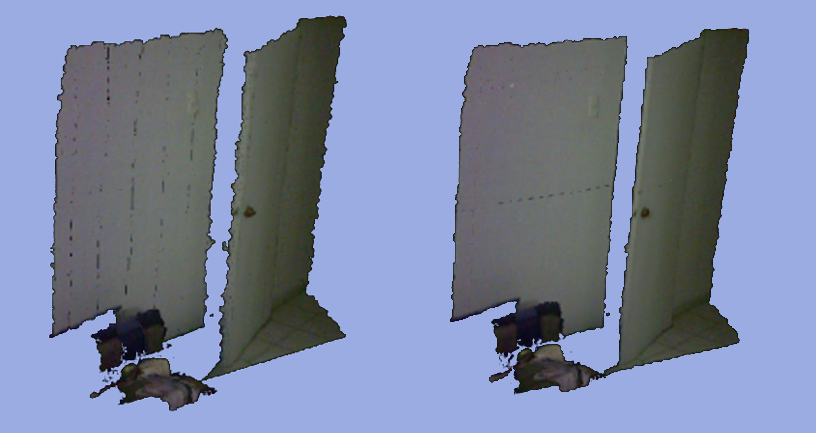
\includegraphics[scale=0.25]{images/bilateral}
\end{center}
\caption{Left: Point cloud without filtering Right: Point cloud with bilateral filtering. Noticeable effects at first sight next to the borders of objects}
\end{figure}

